% Options for packages loaded elsewhere
\PassOptionsToPackage{unicode}{hyperref}
\PassOptionsToPackage{hyphens}{url}
%
\documentclass[
]{article}
\usepackage{amsmath,amssymb}
\usepackage{lmodern}
\usepackage{ifxetex,ifluatex}
\ifnum 0\ifxetex 1\fi\ifluatex 1\fi=0 % if pdftex
  \usepackage[T1]{fontenc}
  \usepackage[utf8]{inputenc}
  \usepackage{textcomp} % provide euro and other symbols
\else % if luatex or xetex
  \usepackage{unicode-math}
  \defaultfontfeatures{Scale=MatchLowercase}
  \defaultfontfeatures[\rmfamily]{Ligatures=TeX,Scale=1}
\fi
% Use upquote if available, for straight quotes in verbatim environments
\IfFileExists{upquote.sty}{\usepackage{upquote}}{}
\IfFileExists{microtype.sty}{% use microtype if available
  \usepackage[]{microtype}
  \UseMicrotypeSet[protrusion]{basicmath} % disable protrusion for tt fonts
}{}
\makeatletter
\@ifundefined{KOMAClassName}{% if non-KOMA class
  \IfFileExists{parskip.sty}{%
    \usepackage{parskip}
  }{% else
    \setlength{\parindent}{0pt}
    \setlength{\parskip}{6pt plus 2pt minus 1pt}}
}{% if KOMA class
  \KOMAoptions{parskip=half}}
\makeatother
\usepackage{xcolor}
\IfFileExists{xurl.sty}{\usepackage{xurl}}{} % add URL line breaks if available
\IfFileExists{bookmark.sty}{\usepackage{bookmark}}{\usepackage{hyperref}}
\hypersetup{
  pdftitle={Aflevering 8},
  hidelinks,
  pdfcreator={LaTeX via pandoc}}
\urlstyle{same} % disable monospaced font for URLs
\usepackage[margin=1in]{geometry}
\usepackage{color}
\usepackage{fancyvrb}
\newcommand{\VerbBar}{|}
\newcommand{\VERB}{\Verb[commandchars=\\\{\}]}
\DefineVerbatimEnvironment{Highlighting}{Verbatim}{commandchars=\\\{\}}
% Add ',fontsize=\small' for more characters per line
\usepackage{framed}
\definecolor{shadecolor}{RGB}{248,248,248}
\newenvironment{Shaded}{\begin{snugshade}}{\end{snugshade}}
\newcommand{\AlertTok}[1]{\textcolor[rgb]{0.94,0.16,0.16}{#1}}
\newcommand{\AnnotationTok}[1]{\textcolor[rgb]{0.56,0.35,0.01}{\textbf{\textit{#1}}}}
\newcommand{\AttributeTok}[1]{\textcolor[rgb]{0.77,0.63,0.00}{#1}}
\newcommand{\BaseNTok}[1]{\textcolor[rgb]{0.00,0.00,0.81}{#1}}
\newcommand{\BuiltInTok}[1]{#1}
\newcommand{\CharTok}[1]{\textcolor[rgb]{0.31,0.60,0.02}{#1}}
\newcommand{\CommentTok}[1]{\textcolor[rgb]{0.56,0.35,0.01}{\textit{#1}}}
\newcommand{\CommentVarTok}[1]{\textcolor[rgb]{0.56,0.35,0.01}{\textbf{\textit{#1}}}}
\newcommand{\ConstantTok}[1]{\textcolor[rgb]{0.00,0.00,0.00}{#1}}
\newcommand{\ControlFlowTok}[1]{\textcolor[rgb]{0.13,0.29,0.53}{\textbf{#1}}}
\newcommand{\DataTypeTok}[1]{\textcolor[rgb]{0.13,0.29,0.53}{#1}}
\newcommand{\DecValTok}[1]{\textcolor[rgb]{0.00,0.00,0.81}{#1}}
\newcommand{\DocumentationTok}[1]{\textcolor[rgb]{0.56,0.35,0.01}{\textbf{\textit{#1}}}}
\newcommand{\ErrorTok}[1]{\textcolor[rgb]{0.64,0.00,0.00}{\textbf{#1}}}
\newcommand{\ExtensionTok}[1]{#1}
\newcommand{\FloatTok}[1]{\textcolor[rgb]{0.00,0.00,0.81}{#1}}
\newcommand{\FunctionTok}[1]{\textcolor[rgb]{0.00,0.00,0.00}{#1}}
\newcommand{\ImportTok}[1]{#1}
\newcommand{\InformationTok}[1]{\textcolor[rgb]{0.56,0.35,0.01}{\textbf{\textit{#1}}}}
\newcommand{\KeywordTok}[1]{\textcolor[rgb]{0.13,0.29,0.53}{\textbf{#1}}}
\newcommand{\NormalTok}[1]{#1}
\newcommand{\OperatorTok}[1]{\textcolor[rgb]{0.81,0.36,0.00}{\textbf{#1}}}
\newcommand{\OtherTok}[1]{\textcolor[rgb]{0.56,0.35,0.01}{#1}}
\newcommand{\PreprocessorTok}[1]{\textcolor[rgb]{0.56,0.35,0.01}{\textit{#1}}}
\newcommand{\RegionMarkerTok}[1]{#1}
\newcommand{\SpecialCharTok}[1]{\textcolor[rgb]{0.00,0.00,0.00}{#1}}
\newcommand{\SpecialStringTok}[1]{\textcolor[rgb]{0.31,0.60,0.02}{#1}}
\newcommand{\StringTok}[1]{\textcolor[rgb]{0.31,0.60,0.02}{#1}}
\newcommand{\VariableTok}[1]{\textcolor[rgb]{0.00,0.00,0.00}{#1}}
\newcommand{\VerbatimStringTok}[1]{\textcolor[rgb]{0.31,0.60,0.02}{#1}}
\newcommand{\WarningTok}[1]{\textcolor[rgb]{0.56,0.35,0.01}{\textbf{\textit{#1}}}}
\usepackage{graphicx}
\makeatletter
\def\maxwidth{\ifdim\Gin@nat@width>\linewidth\linewidth\else\Gin@nat@width\fi}
\def\maxheight{\ifdim\Gin@nat@height>\textheight\textheight\else\Gin@nat@height\fi}
\makeatother
% Scale images if necessary, so that they will not overflow the page
% margins by default, and it is still possible to overwrite the defaults
% using explicit options in \includegraphics[width, height, ...]{}
\setkeys{Gin}{width=\maxwidth,height=\maxheight,keepaspectratio}
% Set default figure placement to htbp
\makeatletter
\def\fps@figure{htbp}
\makeatother
\setlength{\emergencystretch}{3em} % prevent overfull lines
\providecommand{\tightlist}{%
  \setlength{\itemsep}{0pt}\setlength{\parskip}{0pt}}
\setcounter{secnumdepth}{-\maxdimen} % remove section numbering
\ifluatex
  \usepackage{selnolig}  % disable illegal ligatures
\fi

\title{Aflevering 8}
\usepackage{etoolbox}
\makeatletter
\providecommand{\subtitle}[1]{% add subtitle to \maketitle
  \apptocmd{\@title}{\par {\large #1 \par}}{}{}
}
\makeatother
\subtitle{Lucas Bagge}
\author{}
\date{\vspace{-2.5em}}

\begin{document}
\maketitle

\hypertarget{section}{%
\subsection{3.5}\label{section}}

I denne opgave skal I bruge en lineær regressionsmodel til at sige noget
om værdien af den forklarende variabel ud fra en målt responsværdi. I
opgaven her er den forklarende variabel alderen af en løve, og respons
er fraktion af sort pigment i løvens næsetip.

I artiklen Sustainable trophy hunting of African lions diskuteres
hvordan trofæjagt af løver kan gøres bæredygtigt. Forfatternes
konklusion er, at man skal sørge for, at de løver, der jages, er
hanløver over en vis alder. Ofte bruger jægeren størelsen og farven af
løvens manke til at vurdere alderen, men dette er en meget usikker
metode. En mere sikker metode består i at bruge andelen af sort pigment
i løvens næsetip. I opgaven her skal I se på, hvordan andelen af sort
pigment afhænger af alderen, og hvor godt vi kan estimere alderen ud fra
dette.

Data for 32 hanløver fra Serengeti og Ngorongoro nationalparkerne ligger
i filen Loeve.csv, der har to søjler med henholdsvis alder (år) og
fraktion af sort.

Indlæs data:

\begin{Shaded}
\begin{Highlighting}[]
\NormalTok{data }\OtherTok{\textless{}{-}} \FunctionTok{read.csv}\NormalTok{(}\StringTok{"MatStat{-}R/data/JLJfiler/Loeve.csv"}\NormalTok{) }\SpecialCharTok{\%\textgreater{}\%} 
\NormalTok{  janitor}\SpecialCharTok{::}\FunctionTok{clean\_names}\NormalTok{() }
\FunctionTok{head}\NormalTok{(data)}
\end{Highlighting}
\end{Shaded}

\begin{verbatim}
##   alder sortfraktion
## 1   1.1         0.21
## 2   1.5         0.14
## 3   1.9         0.11
## 4   2.2         0.13
## 5   2.6         0.12
## 6   3.2         0.13
\end{verbatim}

\hypertarget{a-lav-en-figur-hvor-fraktion-af-sort-afsuxe6ttes-mod-alder.-styr-start-og-slut-puxe5-andenaksen-med-tilfuxf8jelsen-ylimc01-til-plot.-synes-du-at-der-er-en-lineuxe6r-sammenhuxe6ng-i-data-synes-du-at-sammenhuxe6ngen-er-god-med-henblik-puxe5-at-estimere-alder-ud-fra-fraktion-af-sort-i-nuxe6stippen}{%
\paragraph{a) Lav en figur, hvor fraktion af sort afsættes mod alder.
Styr start og slut på andenaksen med tilføjelsen ylim=c(0,1) til plot.
Synes du, at der er en lineær sammenhæng i data? Synes du, at
sammenhængen er god med henblik på at estimere alder ud fra fraktion af
sort i
næstippen?}\label{a-lav-en-figur-hvor-fraktion-af-sort-afsuxe6ttes-mod-alder.-styr-start-og-slut-puxe5-andenaksen-med-tilfuxf8jelsen-ylimc01-til-plot.-synes-du-at-der-er-en-lineuxe6r-sammenhuxe6ng-i-data-synes-du-at-sammenhuxe6ngen-er-god-med-henblik-puxe5-at-estimere-alder-ud-fra-fraktion-af-sort-i-nuxe6stippen}}

Jeg laver et scatter plot.

\begin{Shaded}
\begin{Highlighting}[]
\FunctionTok{attach}\NormalTok{(data)}
\FunctionTok{plot}\NormalTok{(alder, sortfraktion, }\AttributeTok{ylim =} \FunctionTok{c}\NormalTok{(}\DecValTok{0}\NormalTok{,}\DecValTok{1}\NormalTok{))}
\end{Highlighting}
\end{Shaded}

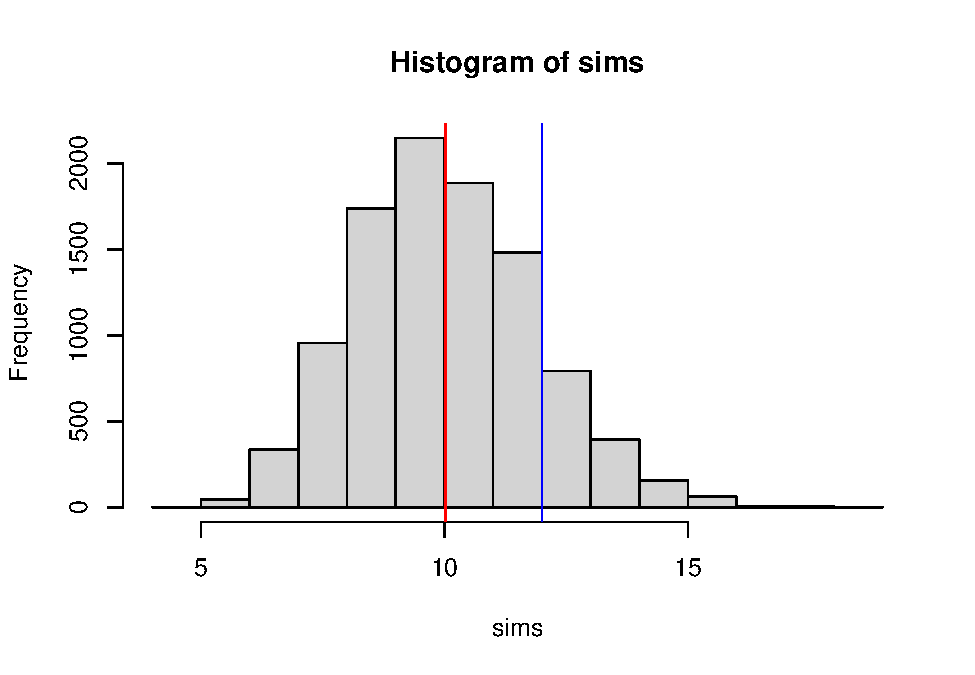
\includegraphics{Aflevering8-skabelon_files/figure-latex/unnamed-chunk-2-1.pdf}

Hvis vi ser fra vores bog \emph{Mathematical statistic with resampling
and R} på side 39, så ser der ud til at være en positiv lineær
sammenhæng og vi kan dermed godt estimere alder ud fra fraktion af sort
i næsetippen.

\hypertarget{b-opskriv-den-lineuxe6re-regressionsmodel-hvor-respons-er-fraktion-af-sort-i-nuxe6setippen-og-den-forklarende-variabel-er-alder.-find-skuxf8n-og-95-konfidensinterval-for-huxe6ldning-og-skuxe6ring-og-indtegn-den-skuxf8nnede-linje-i-figuren-fra-foreguxe5ende-spuxf8rgsmuxe5l.-angiv-ogsuxe5-et-skuxf8n-over-spredningen-sigma-omkring-den-lineuxe6re-sammenhuxe6ng.-lav-figurer-der-kan-bruges-til-modelkontrol-og-kommenter-puxe5-disse-figurer.}{%
\paragraph{\texorpdfstring{b) Opskriv den lineære regressionsmodel, hvor
respons er fraktion af sort i næsetippen, og den forklarende variabel er
alder. Find skøn og 95\%-konfidensinterval for hældning og skæring, og
indtegn den skønnede linje i figuren fra foregående spørgsmål. Angiv
også et skøn over spredningen \(\sigma\) omkring den lineære sammenhæng.
Lav figurer, der kan bruges til modelkontrol, og kommenter på disse
figurer.}{b) Opskriv den lineære regressionsmodel, hvor respons er fraktion af sort i næsetippen, og den forklarende variabel er alder. Find skøn og 95\%-konfidensinterval for hældning og skæring, og indtegn den skønnede linje i figuren fra foregående spørgsmål. Angiv også et skøn over spredningen \textbackslash sigma omkring den lineære sammenhæng. Lav figurer, der kan bruges til modelkontrol, og kommenter på disse figurer.}}\label{b-opskriv-den-lineuxe6re-regressionsmodel-hvor-respons-er-fraktion-af-sort-i-nuxe6setippen-og-den-forklarende-variabel-er-alder.-find-skuxf8n-og-95-konfidensinterval-for-huxe6ldning-og-skuxe6ring-og-indtegn-den-skuxf8nnede-linje-i-figuren-fra-foreguxe5ende-spuxf8rgsmuxe5l.-angiv-ogsuxe5-et-skuxf8n-over-spredningen-sigma-omkring-den-lineuxe6re-sammenhuxe6ng.-lav-figurer-der-kan-bruges-til-modelkontrol-og-kommenter-puxe5-disse-figurer.}}

Den lineære regressions model vil være følgende:

\[
sortfraktion = \alpha + alder \cdot x
\]

Implementerin i R:

\begin{Shaded}
\begin{Highlighting}[]
\NormalTok{model }\OtherTok{\textless{}{-}} \FunctionTok{lm}\NormalTok{(sortfraktion }\SpecialCharTok{\textasciitilde{}}\NormalTok{ alder, }\AttributeTok{data =}\NormalTok{ data)}
\NormalTok{sumUD }\OtherTok{\textless{}{-}} \FunctionTok{summary}\NormalTok{(model)}
\NormalTok{sumUD}
\end{Highlighting}
\end{Shaded}

\begin{verbatim}
## 
## Call:
## lm(formula = sortfraktion ~ alder, data = data)
## 
## Residuals:
##      Min       1Q   Median       3Q      Max 
## -0.20406 -0.07758 -0.01750  0.07913  0.29876 
## 
## Coefficients:
##             Estimate Std. Error t value Pr(>|t|)    
## (Intercept) 0.069696   0.041956   1.661    0.107    
## alder       0.058591   0.008307   7.053 7.68e-08 ***
## ---
## Signif. codes:  0 '***' 0.001 '**' 0.01 '*' 0.05 '.' 0.1 ' ' 1
## 
## Residual standard error: 0.1238 on 30 degrees of freedom
## Multiple R-squared:  0.6238, Adjusted R-squared:  0.6113 
## F-statistic: 49.75 on 1 and 30 DF,  p-value: 7.677e-08
\end{verbatim}

Hvor skøn for skæring er: 0.069696 mens den for hældning er 0.041956.

Vi kan burge \texttt{confint} til at finde konfidens intervallet.

\begin{Shaded}
\begin{Highlighting}[]
\FunctionTok{confint}\NormalTok{(model)}
\end{Highlighting}
\end{Shaded}

\begin{verbatim}
##                   2.5 %     97.5 %
## (Intercept) -0.01598977 0.15538230
## alder        0.04162643 0.07555588
\end{verbatim}

Herefter skal vi tegne vores skøn ind:

\begin{Shaded}
\begin{Highlighting}[]
\FunctionTok{plot}\NormalTok{(alder, sortfraktion, }\AttributeTok{ylim =} \FunctionTok{c}\NormalTok{(}\DecValTok{0}\NormalTok{,}\DecValTok{1}\NormalTok{))}
\FunctionTok{abline}\NormalTok{(model, }\AttributeTok{col =} \StringTok{"red"}\NormalTok{)}
\end{Highlighting}
\end{Shaded}

\includegraphics{Aflevering8-skabelon_files/figure-latex/unnamed-chunk-5-1.pdf}

Så skal vi angive skønnet over spredning, \(s_r\):

\begin{Shaded}
\begin{Highlighting}[]
\NormalTok{sumUD}\SpecialCharTok{$}\NormalTok{sigma}
\end{Highlighting}
\end{Shaded}

\begin{verbatim}
## [1] 0.1237927
\end{verbatim}

Så for modelkontrol

\begin{Shaded}
\begin{Highlighting}[]
\NormalTok{model\_res }\OtherTok{\textless{}{-}} \FunctionTok{resid}\NormalTok{(model)}
\FunctionTok{par}\NormalTok{(}\AttributeTok{mfrow=}\FunctionTok{c}\NormalTok{(}\DecValTok{1}\NormalTok{,}\DecValTok{2}\NormalTok{))}
\FunctionTok{plot}\NormalTok{(data}\SpecialCharTok{$}\NormalTok{alder,model\_res)}
\FunctionTok{abline}\NormalTok{(}\DecValTok{0}\NormalTok{,}\DecValTok{0}\NormalTok{)}
\FunctionTok{qqnorm}\NormalTok{(model\_res)}
\end{Highlighting}
\end{Shaded}

\includegraphics{Aflevering8-skabelon_files/figure-latex/unnamed-chunk-7-1.pdf}

Residualplotter tyder ikke på afvigelser fra en lineære sammenhæng. Kun
vi en outlier måske med den ydersste observation. QQplottet giver ikke
anledning til bekymring med hensyn til normalfordelingsantagelsen.

\hypertarget{c-betragt-situationen-hvor-en-ny-luxf8ve-registreres-og-fraktion-af-sort-i-nuxe6sen-for-denne-luxf8ve-er-0.2.-beregn-et-95-konfidensinterval-for-luxf8vens-alder-i-dette-tilfuxe6lde.-gentag-beregningen-i-tre-andre-tilfuxe6lde-hvor-en-luxf8ve-er-observeret-med-henholdsvis-0.4-0.6-og-0.8-for-fraktionen-af-sort-i-nuxe6sen.-lav-en-tabel-med-resultaterne-for-de-fire-tilfuxe6lde.-hvis-vi-kun-uxf8nsker-at-skyde-luxf8ver-der-er-mindst-5-uxe5r-gamle-hvor-stor-synes-du-suxe5-fraktionen-af-sort-i-nuxe6sen-skal-vuxe6re-fuxf8r-du-skyder}{%
\paragraph{c) Betragt situationen, hvor en ny løve registreres, og
fraktion af sort i næsen for denne løve er 0.2. Beregn et
95\%-konfidensinterval for løvens alder i dette tilfælde. Gentag
beregningen i tre andre tilfælde, hvor en løve er observeret med
henholdsvis 0.4, 0.6 og 0.8 for fraktionen af sort i næsen. Lav en tabel
med resultaterne for de fire tilfælde. Hvis vi kun ønsker at skyde
løver, der er mindst 5 år gamle, hvor stor synes du så fraktionen af
sort i næsen skal være, før du
skyder?}\label{c-betragt-situationen-hvor-en-ny-luxf8ve-registreres-og-fraktion-af-sort-i-nuxe6sen-for-denne-luxf8ve-er-0.2.-beregn-et-95-konfidensinterval-for-luxf8vens-alder-i-dette-tilfuxe6lde.-gentag-beregningen-i-tre-andre-tilfuxe6lde-hvor-en-luxf8ve-er-observeret-med-henholdsvis-0.4-0.6-og-0.8-for-fraktionen-af-sort-i-nuxe6sen.-lav-en-tabel-med-resultaterne-for-de-fire-tilfuxe6lde.-hvis-vi-kun-uxf8nsker-at-skyde-luxf8ver-der-er-mindst-5-uxe5r-gamle-hvor-stor-synes-du-suxe5-fraktionen-af-sort-i-nuxe6sen-skal-vuxe6re-fuxf8r-du-skyder}}

Nu lader vi som om vi observer en ny løve der har en sort fraktion på
0.2. Hertil laver jeg et nyt datasæt.

\begin{Shaded}
\begin{Highlighting}[]
\NormalTok{new\_data }\OtherTok{\textless{}{-}} \FunctionTok{data.frame}\NormalTok{(}
  \AttributeTok{sortfraktion =} \FloatTok{0.2}
\NormalTok{)}
\end{Highlighting}
\end{Shaded}

Nu skal vi altså forudsige hvad alderen på den nye løve er når den har
en sortfraktion på 0.2. Hertil laver vi en ny model hvor vi regresser
alder på sortfraktion og bruger R prediction til at lave denne analyse:

\begin{Shaded}
\begin{Highlighting}[]
\FunctionTok{source}\NormalTok{(}\StringTok{"MatStat{-}R/source/Rfunktioner.R"}\NormalTok{)}
\FunctionTok{inversReg}\NormalTok{(model, new\_data}\SpecialCharTok{$}\NormalTok{sortfraktion)}
\end{Highlighting}
\end{Shaded}

\begin{verbatim}
## $estimat
## [1] 2.223949
## 
## $konfidensinterval
## [1] -2.592041  6.658276
\end{verbatim}

Her ser vi at løven burde være 3 år indenfor 2.29 og 3.7.

Nu får vi yderligere tre nye løver hvor vi skal lave samme analyse. Her
kobler jeg bare alle fire på, da vi bliver bedt om at lave en tabel:

\begin{Shaded}
\begin{Highlighting}[]
\NormalTok{new\_data }\OtherTok{\textless{}{-}} \FunctionTok{data.frame}\NormalTok{(}
  \AttributeTok{sortfraktion =} \FunctionTok{c}\NormalTok{(}\FloatTok{0.2}\NormalTok{, }\FloatTok{0.4}\NormalTok{, }\FloatTok{0.6}\NormalTok{, }\FloatTok{0.8}\NormalTok{)}
\NormalTok{)}
\FunctionTok{inversReg}\NormalTok{(model, new\_data}\SpecialCharTok{$}\NormalTok{sortfraktion)}
\end{Highlighting}
\end{Shaded}

\begin{verbatim}
## $estimat
## [1] 7.344176
## 
## $konfidensinterval
## [1]  5.045909 10.197858
\end{verbatim}

Her til sidst skal vi så svarer på hvad fraktionen af sort skal være før
vi vil skyde en løve på baggrund af den er mindst 5 år. Ud fra vores
prediction så skal skal en løve have omkring 0.4 fraktion så vil den
være omkring 5 år.

Kigger vi dog på selve data:

\begin{Shaded}
\begin{Highlighting}[]
\FunctionTok{library}\NormalTok{(dplyr)}
\end{Highlighting}
\end{Shaded}

\begin{verbatim}
## Warning: package 'dplyr' was built under R version 4.0.4
\end{verbatim}

\begin{verbatim}
## 
## Attaching package: 'dplyr'
\end{verbatim}

\begin{verbatim}
## The following objects are masked from 'package:stats':
## 
##     filter, lag
\end{verbatim}

\begin{verbatim}
## The following objects are masked from 'package:base':
## 
##     intersect, setdiff, setequal, union
\end{verbatim}

\begin{Shaded}
\begin{Highlighting}[]
\NormalTok{data }\SpecialCharTok{\%\textgreater{}\%} 
  \FunctionTok{filter}\NormalTok{(alder }\SpecialCharTok{\textgreater{}} \FloatTok{5.0}\NormalTok{)}
\end{Highlighting}
\end{Shaded}

\begin{verbatim}
##    alder sortfraktion
## 1    5.4         0.59
## 2    5.8         0.60
## 3    6.0         0.72
## 4    7.3         0.48
## 5    7.3         0.44
## 6    7.8         0.34
## 7    7.1         0.37
## 8    7.1         0.34
## 9   13.1         0.74
## 10   8.8         0.79
## 11   5.4         0.51
\end{verbatim}

Foroven laver jeg et filter på mit data og ser at mange løver som er
omkring 5 til 6 år har en sortfraktion på 0.5 til 0.7, som giver god
mening ud fra vores model prediction, men ser vi på alderen 7, så har
den en sortfraktion på under 0.5, og det er misvisende for så tyder det
på at vi har nogle løver som er gammel men ikke har meget fraktion på
næsen.

Derfor er vores model ikke særlig god og jeg tør ikke udtale mig om hvad
fraktionen skal være for vi vil skyde en løve som er mindst 5 år.

\end{document}
